%% ======================================================================
%% Artículo EXPOTIC UNAB 2026 — Formato UNAB
%% Arial 12 (helvet), interlineado 1.15, márgenes 2.5 cm,
%% portada a 1 columna, cuerpo a 2 columnas, citas APA (autor, año).
%% Compilar: pdflatex -> bibtex -> pdflatex -> pdflatex
%%           (o: latexmk -pdf articulo.tex)
%% ======================================================================
\documentclass[12pt]{article}

\usepackage[utf8]{inputenc}
\usepackage[T1]{fontenc}
\usepackage[spanish,es-nodecimaldot,es-tabla]{babel}
\usepackage[margin=2.5cm]{geometry}
\usepackage{helvet}                     % Arial (equivalente)
\renewcommand{\familydefault}{\sfdefault}
\usepackage{setspace}
\setstretch{1.15}                       % interlineado 1.15
\usepackage{amsmath,amssymb}
\usepackage{booktabs,multirow}
\usepackage{graphicx}
\graphicspath{{figuras/}}
\usepackage[round]{natbib}              % citas (Autor, año) — APA
\usepackage{url}
\usepackage[hidelinks]{hyperref}
\usepackage{caption}
\captionsetup{font=small,labelfont=bf}
\usepackage{enumitem}
\setlist{itemsep=1pt,topsep=3pt,parsep=0pt}
\setlength{\columnsep}{0.8cm}
\setlength{\parindent}{0.6cm}

\newcommand{\NP}{\ensuremath{\mathcal{NP}}}

\begin{document}

%% ------------------- PORTADA A 1 COLUMNA (página propia) -------------
\begin{center}
  
\includegraphics[width=3.9cm]{logo_articulo}\\[0.3cm]
  {\Large\bfseries Triple Enfoque Resolutivo: Un Repositorio de Cinco
   Problemas de Optimización Combinatoria con Soluciones Exactas y
   Metaheurísticas\par}
  \vspace{0.3cm}
  {\large Peña Díaz, Benjamín (Autor) \; · \;
          Gatica, Gustavo (Profesor Guía)\par}
  \vspace{0.15cm}
  Universidad Andrés Bello -- Facultad de Ingeniería \; \textbar{} \;
  Ingeniería Civil Informática\\
  Santiago de Chile, Julio 2026 \; \textbar{} \;
  \texttt{benja.diaz.2911@gmail.com} \; · \; \texttt{ggatica@unab.cl}
  \vspace{0.35cm}
\end{center}

%% ------------------- RESUMEN / ABSTRACT (apilados) --------------------
\begin{center}\textbf{Resumen}\end{center}
\vspace{-0.15cm}
{\footnotesize\setstretch{1.1}
\noindent
Se presenta un repositorio reproducible para la evaluación comparativa de
metaheurísticas en cinco problemas clásicos de optimización combinatoria:
mochila 0/1 (\textit{Knapsack}), problema del viajante (TSP), ruteo de
vehículos con capacidad (CVRP), \textit{Permutation Flowshop} y
\textit{Job Shop}. Para cada problema se implementaron tres configuraciones
progresivas de Búsqueda Tabú (TS): básica (lista tabú fija), intermedia
(lista dinámica con aspiración y reinicio suave) y avanzada (memoria de
frecuencia, penalización adaptativa y diversificación informada). Los 360
experimentos ejecutados sobre benchmarks clásicos (TSPLIB, Pisinger,
Christofides, Taillard, OR-Library), con cinco semillas independientes por
configuración, muestran que TS-Avanzado reduce el GAP global promedio
respecto al mejor valor conocido (BKS) de 6.22\,\% a 3.06\,\%, con mejoras
especialmente notorias en CVRP (19.22\,\% $\rightarrow$ 6.38\,\%) y TSP
(2.42\,\% $\rightarrow$ 1.22\,\%). El repositorio incluye cargadores de
instancias, modelos exactos de referencia, un orquestador de experimentos y
generadores de tablas, para facilitar la replicación y extensión de los
resultados.

\vspace{0.1cm}
\noindent
\textbf{Palabras clave:} búsqueda tabú, optimización combinatoria,
metaheurísticas, repositorio reproducible, GAP.
}

\vspace{0.25cm}
\begin{center}\textbf{Abstract}\end{center}
\vspace{-0.15cm}
{\footnotesize\setstretch{1.1}
\noindent
A reproducible repository is presented for the comparative evaluation of
metaheuristics on five classical combinatorial optimization problems: 0/1
Knapsack, the Traveling Salesman Problem (TSP), the Capacitated Vehicle
Routing Problem (CVRP), Permutation Flowshop Scheduling, and Job Shop
Scheduling. For each problem, three progressive Tabu Search (TS)
configurations were implemented: basic (fixed tabu list), intermediate
(dynamic list with aspiration and soft restart), and advanced (frequency
memory, adaptive penalization, and informed diversification). The 360
experiments executed on classical benchmarks (TSPLIB, Pisinger,
Christofides, Taillard, OR-Library), with five independent seeds per
configuration, show that Advanced TS reduces the global average GAP with
respect to the best known solution (BKS) from 6.22\,\% to 3.06\,\%, with
particularly notable improvements in CVRP (19.22\,\% $\rightarrow$
6.38\,\%) and TSP (2.42\,\% $\rightarrow$ 1.22\,\%). The repository
includes instance loaders, exact reference models, an experiment
orchestrator, and table generators to facilitate replication and extension
of the results.

\vspace{0.1cm}
\noindent
\textbf{Keywords:} tabu search, combinatorial optimization, metaheuristics,
reproducible repository, GAP.
}

%% ------------------- CUERPO A 2 COLUMNAS -----------------------------
\twocolumn

\section{Introducción}

Los problemas de optimización combinatoria (POC) aparecen en áreas tan
diversas como logística, manufactura, finanzas y planificación de recursos.
Su complejidad computacional, mayoritariamente \NP-dura
\citep{garey1979computers}, ha impulsado el desarrollo de algoritmos
exactos y, especialmente, de metaheurísticas capaces de obtener soluciones
de buena calidad en tiempos prácticos \citep{gendreau2010handbook}.

La Búsqueda Tabú (TS), propuesta por \citet{glover1986future,glover1989tabu},
registra movimientos recientes en una lista tabú para evitar la re-visita de
soluciones y escapar de óptimos locales, y puede enriquecerse con memoria
de largo plazo, criterios de aspiración, reinicios y penalizaciones
adaptativas \citep{glover1997tabu}.

La mayoría de los estudios compara TS contra otras familias
---algoritmos genéticos \citep{holland1975adaptation}, recocido simulado
\citep{kirkpatrick1983optimization} u optimización por colonias de hormigas
\citep{dorigo1996ant}--- o propone variantes altamente especializadas para
un único problema. Existe una brecha metodológica: faltan repositorios
públicos que ilustren la \emph{progresión interna} de TS ---de una
configuración básica a una avanzada--- sobre múltiples problemas
heterogéneos, con código reproducible y métricas unificadas.

El objetivo general de este trabajo es construir y validar un repositorio
abierto que cuantifique el aporte incremental de cada mecanismo de TS en
cinco POC clásicos. Las contribuciones son: (1) quince módulos de TS en
Python (5 problemas $\times$ 3 configuraciones) con interfaz uniforme;
(2) un orquestador que ejecuta los 360 experimentos de forma automatizada;
(3) un análisis cuantitativo del impacto de la memoria de frecuencia, la
lista tabú dinámica y la diversificación adaptativa; y (4) un repositorio
extensible a nuevos problemas o algoritmos.

\section{Metodología}

\subsection{Problemas abordados}

Se estudian cinco POC clásicos en sus formulaciones estándar: la mochila
0/1 \citep{martello1990knapsack}, el TSP en la formulación de
\citet{dantzig1954solution}, el CVRP \citep{laporte1992vehicle}, el
\textit{Permutation Flowshop} \citep{pinedo2016scheduling} y el
\textit{Job Shop} \citep{garey1976complexity}. Todos son \NP-duros y
cuentan con benchmarks públicos con mejores valores conocidos (BKS).

\subsection{Tres niveles de Búsqueda Tabú}

Cada nivel incorpora los componentes del anterior y añade nuevos, lo que
permite aislar la contribución de cada mecanismo:

\begin{itemize}
  \item \textbf{TS-Básico:} lista tabú de tamaño fijo y vecindario
    estándar (flip de bit en Knapsack, 2-opt en TSP
    \citep{lin1973effective}, reubicación en CVRP, swap adyacente en
    Flowshop y Job Shop).
  \item \textbf{TS-Intermedio:} lista tabú dinámica, criterio de
    aspiración y reinicio suave tras $L$ iteraciones sin mejora.
  \item \textbf{TS-Avanzado:} memoria de frecuencia, penalización
    adaptativa y diversificación informada; en TSP incorpora la
    perturbación \textit{double-bridge} (4-opt)
    \citep{johnson1997traveling}.
\end{itemize}

\subsection{Instancias y soluciones iniciales}

Se emplearon 24 instancias de benchmarks clásicos: Pisinger para Knapsack
\citep{pisinger2005hard}, TSPLIB \citep{reinelt1991tsplib}, Christofides
para CVRP \citep{christofides1979vehicle}, Taillard para Flowshop
\citep{taillard1993benchmarks} y Fisher--Thompson/Lawrence para Job Shop
\citep{fisher1963probabilistic,lawrence1984resource}. Las soluciones
iniciales se construyen con heurísticas específicas: greedy por ratio en
Knapsack, vecino más cercano en TSP, ahorros de Clarke--Wright en CVRP
\citep{clarke1964scheduling}, NEH en Flowshop \citep{nawaz1983heuristic} y
Giffler--Thompson en Job Shop \citep{giffler1960algorithms}.

\subsection{Diseño experimental y métricas}

Se ejecutaron 360 experimentos (24 instancias $\times$ 3 algoritmos
$\times$ 5 semillas independientes). El rendimiento se mide con el GAP
porcentual respecto al BKS:

\begin{equation}
  \text{GAP}(\%) = \frac{|f^{*} - \text{BKS}|_{\text{signo}}}{\text{BKS}}
  \times 100,
  \label{eq:gap}
\end{equation}

\noindent
donde $f^{*}$ es el mejor valor hallado y el signo se ajusta según se trate
de minimización o maximización. Un GAP negativo indica que se superó el
BKS publicado. Se reportan media y desviación estándar sobre las cinco
semillas $s \in \{42, 123, 456, 789, 1337\}$. Los experimentos se
ejecutaron en un equipo con procesador Intel Core i7 (11.ª generación) y
8~GB de RAM.

\section{Resultados}

La Tabla~\ref{tab:consolidada} sintetiza el GAP promedio y el tiempo medio
por problema y nivel de TS.

\begin{table}[t]
\caption{GAP promedio (\%) y tiempo promedio (s) por problema y algoritmo
         (media sobre 5 semillas).}
\label{tab:consolidada}
\centering
\small
\setlength{\tabcolsep}{3pt}
\begin{tabular}{lcccccc}
\toprule
 & \multicolumn{2}{c}{\textbf{Básico}}
 & \multicolumn{2}{c}{\textbf{Intermedio}}
 & \multicolumn{2}{c}{\textbf{Avanzado}} \\
\cmidrule(lr){2-3}\cmidrule(lr){4-5}\cmidrule(lr){6-7}
\textbf{Problema} & GAP & T(s) & GAP & T(s) & GAP & T(s) \\
\midrule
Knapsack  & 0.22  & 0.01  & 0.13 & 0.02 & 0.10 & 0.07 \\
TSP       & 2.42  & 1.91  & 2.15 & 4.09 & 1.22 & 8.39 \\
CVRP      & 19.22 & 2.93  & 7.72 & 9.21 & 6.38 & 69.25 \\
Flowshop  & 0.37  & 3.96  & 0.44 & 7.89 & 0.05 & 9.75 \\
Job Shop  & 8.89  & 16.05 & 8.24 & 5.91 & 7.52 & 8.68 \\
\midrule
\textbf{Global} & \textbf{6.22} & -- & \textbf{3.74} & -- &
\textbf{3.06} & -- \\
\bottomrule
\end{tabular}
\end{table}

En \textbf{Knapsack} los tres niveles logran GAPs inferiores a 0.7\,\% en
todas las instancias, gracias al vecindario exhaustivo y a la buena
solución inicial. En \textbf{TSP} la mejora más notable proviene de la
perturbación \textit{double-bridge} de TS-Avanzado: en \texttt{kroA100} el
GAP cae de 2.99\,\% a 0.76\,\% (Figura~\ref{fig:conv_tsp}). El
\textbf{CVRP} es el problema donde la progresión tiene mayor impacto: el
GAP promedio baja de 19.22\,\% (Básico) a 6.38\,\% (Avanzado), una
reducción relativa del 67\,\% (Figura~\ref{fig:conv_vrp}). En
\textbf{Flowshop}, la heurística NEH ya entrega soluciones cercanas al
óptimo; TS-Avanzado alcanza GAPs negativos en \texttt{ta001} y
\texttt{ta011}, superando el BKS publicado en 1993. El \textbf{Job Shop}
resulta el problema más difícil: \texttt{ft10} y \texttt{la21} mantienen
GAPs de 16--20\,\%, consistentes con la dificultad conocida de estos
benchmarks.

\begin{figure}[t]
  \centering
  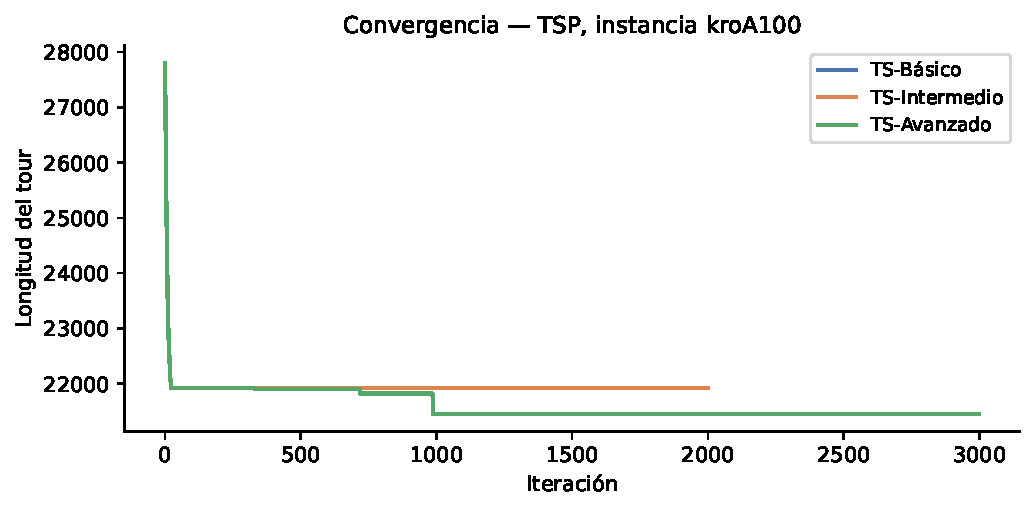
\includegraphics[width=\columnwidth]{convergencia_tsp}
  \caption{Convergencia del GAP (\%) --- TSP, instancia kroA100.}
  \label{fig:conv_tsp}
\end{figure}

\begin{figure}[t]
  \centering
  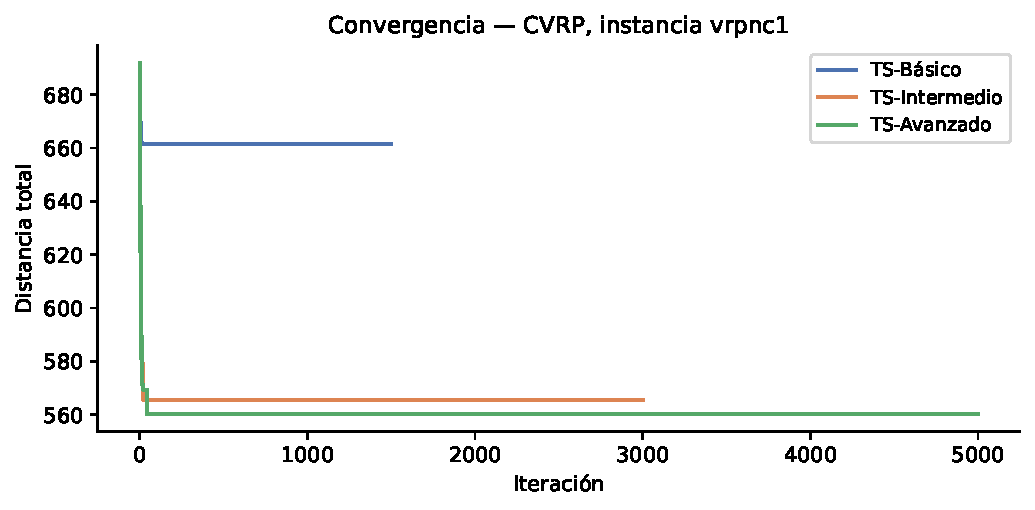
\includegraphics[width=\columnwidth]{convergencia_vrp}
  \caption{Convergencia del GAP (\%) --- CVRP, instancia vrpnc1.}
  \label{fig:conv_vrp}
\end{figure}

El costo computacional crece con el nivel, pero de forma moderada:
TS-Avanzado requiere en promedio $3.9\times$ el tiempo de TS-Básico,
mientras que la reducción del GAP global es del 51\,\% relativo.

\section{Discusión}

Los resultados permiten atribuir el aporte de cada mecanismo. La memoria
de frecuencia y la penalización adaptativa son los componentes de mayor
impacto global, especialmente en CVRP, donde el operador de reubicación
simple de TS-Básico queda atrapado en óptimos locales profundos. La lista
tabú dinámica contribuye modestamente (6.22\,\% $\rightarrow$ 3.74\,\%),
y los mecanismos de largo plazo aportan 0.68~puntos porcentuales
adicionales. La perturbación informada es crítica en TSP, en línea con lo
reportado por \citet{johnson1997traveling} para métodos de reinicio en
búsqueda local. En Flowshop, el margen de mejora es estrecho porque NEH
\citep{nawaz1983heuristic} ya es casi óptima en instancias medianas, y en
Job Shop los GAPs elevados sugieren la necesidad de vecindades más ricas
basadas en el grafo de disyunción \citep{balas1998one}. Se observó además
una inversión puntual en \texttt{vrpnc4} (150 clientes), donde la
penalización adaptativa sobrepondera clientes muy visitados; esto delimita
el alcance de la configuración avanzada en instancias densas.

\section{Conclusiones}

Se construyó y validó un repositorio reproducible con quince
implementaciones de Búsqueda Tabú sobre cinco POC clásicos, cumpliendo el
objetivo de cuantificar el aporte incremental de cada mecanismo
metaheurístico: el GAP global se reduce de 6.22\,\% a 3.06\,\% al pasar de
la configuración básica a la avanzada. Como limitaciones, el presupuesto
de cómputo restringió las iteraciones en instancias grandes de CVRP y Job
Shop, y la comparación usa iteraciones fijas en lugar de tiempo de CPU
fijo. El trabajo futuro contempla incorporar modelos exactos (MILP) como
cotas de referencia, una cuarta configuración poblacional de TS, instancias
de mayor escala y nuevos problemas como coloración de grafos o mochila
multidimensional.

\renewcommand{\refname}{Referencias}
\setlength{\bibsep}{2pt}
\bibliographystyle{apalike-es}
{\footnotesize\setstretch{1.0}
\bibliography{referencias}
}

\end{document}
